\chapter*{¿Dónde debería un piloto iniciar su aterrizaje?}

\begin{wrapfigure}{l}{0.3\textwidth}
	\centering
	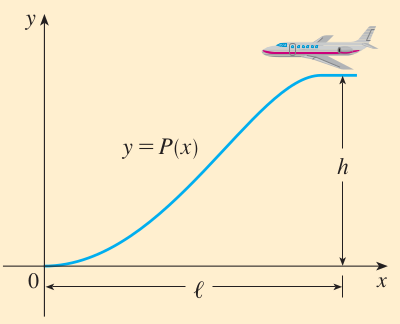
\includegraphics[width = 0.3\textwidth]{recursos/Captura desde 2024-09-21 16-53-03.png}
	\caption{caption}
	\vspace{-60px}
\end{wrapfigure}
En la figura se muestra una trayectoria de aproximación para el aterrizaje de un avión, que satisface las condiciones siguientes:

\begin{enumerate}[label=\Roman*)]
	\item La altura del crucero es $h$ cuando se inicia el descenso a una distancia $l$ del punto de contacto con la pista en el origen.
	\item El piloto debe mantener una rapidez horizontal constante $v$ a todo lo largo del descenso.
	\item El valor absoluto de la aceleración vertical no debe sobrepasar una constante $k$ (la cual es mucho menor que la aceleración debida a la gravedad).
\end{enumerate}

1. Encuentre un polinomio cúbico $P(x)= ax^3+ bx^2 + cx + d$ que satisfaga la condición I), imponiendo condiciones adecuadas sobre $P(x)$ y $P'(x)$ en el inicio del descenso y el contacto con la pista.

\vspace{10pt}

\noindent 2. Use las condiciones I) y III) para demostrar que$$\frac{6hv^2}{l^2}\leq k$$

\vspace{10pt}

\noindent 3. Suponga que una aerolínea comercial decide no permitir que la aceleración vertical de un avión sea mayor que $k = 860 mi/h^2$. Si la altitud de crucero de un avión es de $35 000$ pies y la rapidez de $300 mi/h$, ¿a qué distancia del aeropuerto debe el piloto iniciar el descenso?

\vspace{10pt}

\noindent 4.Trace la grafica de la trayectoria de aproximación si se satisfacen las condiciones que se enuncian en el problema 3.

\textbf{Inciso 1}.- Tenemos las condiciones
\begin{align*}
	P(l)  & =h                                                                       \\
	P(0)  & =0\text{ (Para un aterrizaje suave)}                                     \\
	P'(l) & =0\text{ (debido a que la pendiente en este punto es paralela al eje x)} \\
	P'(0) & =0                                                                       \\
\end{align*}
Primero debemos construir el polinomio de la forma $P(x)= ax^3+ bx^2 + cx + d$ donde su derivada es $P'(x)= 3ax^2+2bx +c$, usando las condiciones

\begin{multicols}{4}
	\noindent
	\begin{align*}
		P(l) & =h:                   \\
		     & al^3+ bl^2 + cl + d=h \\
	\end{align*}
	\columnbreak
	\begin{align*}
		P(0) & =0: \\
		d    & =0  \\
	\end{align*}
	\columnbreak
	\begin{align*}
		P'(l) & =0:            \\
		      & 3al^2+2bl +c=0 \\
	\end{align*}
	\columnbreak
	\begin{align*}
		P'(0) & =0: \\
		      & c=0 \\
	\end{align*}
\end{multicols}

$\implies$ Sustituimos $c$ y $d$ en las ecuaciones y decimos que $P(x)=ax^3+ bx^2 \text{ y } P'(l)= 3al^2+2bl$

Resolviendo para b:
$$b = -\frac{3al^2}{2l} = -\frac{3al}{2}$$
Sustituyendo de $P(l)=h$:
\begin{align*}
	al^3 - \frac{3al^2}{2}l           & = h               \\
	al^3 - \frac{3al^3}{2}            & = h               \\
	al^3 \left(1 - \frac{3}{2}\right) & = h               \\
	al^3 \left(-\frac{1}{2}\right)    & = h               \\
	\therefore a                      & = -\frac{2h}{l^3} \\
\end{align*}

Sustituyendo $a$ en $b$:
\begin{align*}
	a & = -\frac{2h}{l^3}                           \\
	b & = -\frac{3al}{2}                            \\
	  & = -\frac{3}{2}\left(-\frac{2h}{l^3}\right)l \\
	  & = \frac{3h}{l^2}
\end{align*}

Sutituimos la expresión anterior en $P(x)$
$$\implies P(x) = -\frac{2h}{l^3}x^3 + \frac{3h}{l^2}x^2$$

\textbf{Inciso 2}.- Demostrar que $\frac{6hv^2}{l^2} \leq k$

Por el inciso \textbf{II)} nos dice que la velocidad horizontal es constante, $x'(t)=-v, \forall t$ por lo que la posición $x$ en función del tiempo $t$ es: $l-v(t)$ donde $l$ es la distancia al punto de contacto con la pista cuando el descenso comienza, de este modo se asegura que en el transcurso del tiempo $t$ implicará que el crucero efectivamente recorrió la distancia requerida para llegar a la pista de aterrizaje en un tiempo $t$.

El inciso \textbf{III)} dice que el valor absoluto de la aceleración vertical no debe sobrepasar una constante $k$. Establece el límite en la aceleración vertical, por lo que, $\left|\frac{d^2 y}{dt}\right|\leq k$

Primero, calculamos la derivada primera de $y$ respecto a $x$ usando la regla de la cadena:
$$\frac{dy}{dt} = \frac{dy}{dx} \cdot \frac{dx}{dt}$$
Tenemos que $y = P(x) = -\frac{2h}{l^3} x^3 + \frac{3h}{l^2} x^2$, derivamos respecto a $x$
\begin{align*}
	\frac{dy}{dx} & = \frac{d}{dx} \left(-\frac{2h}{l^3} x^3 + \frac{3h}{l^2} x^2 \right) \\
	              & = -\frac{6h}{l^3} x^2 + \frac{6h}{l^2} x
\end{align*}

Dado que tenemos que $\frac{dy}{dt} = \frac{dy}{dx} \cdot \frac{dx}{dt}$ y $\frac{dx}{dt}=-v$, ent:
\begin{align*}
	\frac{dy}{dt} = & \left(-\frac{6h}{l^3} x^2 + \frac{6h}{l^2} x\right) \cdot \frac{dx}{dt}      \\
	=               & -\frac{6h}{l^3} x^2\cdot \frac{dx}{dt} + \frac{6h}{l^2} x\cdot \frac{dx}{dt} \\
	=               & -\frac{6h}{l^3} x^2\cdot (-v) + \frac{6h}{l^2} x\cdot (-v)                   \\
	=               & \frac{6h v x^2}{l^3} - \frac{6h v x}{l^2}
\end{align*}
Derivada Segunda utilizando la Regla de la Cadena
\begin{align*}
	\frac{d^2 y}{d t^2} & = \frac{d}{dx} \left( \frac{6h v x^2}{l^3} - \frac{6h v x}{l^2} \right) \cdot \frac{dx}{dt} \\
	                    & = \frac{d}{dx} \left( \frac{6hvx^2}{l^3} - \frac{6hvx}{l^2} \right) \cdot (-v)              \\
	                    & =  \left(\frac{6hv}{l^3}(2x) - \frac{6hv}{l^2}\right)\cdot (-v)                             \\
	                    & = -\frac{12hv^2x}{l^3} + \frac{6hv^2}{l^2}                                                  \\
\end{align*}

Para obtener la aceleración vertical inicial, evaluamos, en particular, cuando $t = 0$, $x = l$:
\begin{align*}
	\frac{d^2 y}{d t^2} \Bigg|_{t=0}                  & = \frac{-12h v^2 l}{l^3} + \frac{6h v^2}{l^2} \\
	                                                  & = -\frac{12h v^2}{l^2} + \frac{6h v^2}{l^2}   \\
	                                                  & = -\frac{6h v^2}{l^2}                         \\
	\implies \left| \frac{d^2 y}{d t^2} \right|_{t=0} & = \frac{6 h v^2}{l^2}                         \\
	\therefore \frac{6 h v^2}{l^2}                    & \leq  k
\end{align*}
Confirmamos que la aceleración vertical máxima cumple la restricción $\left| \frac{d^2 y}{d t^2} \right| \leq k$

\textbf{Inciso 3}.- Determinación de la distancia de descenso
Sustitución de valores $k = 860 \ \mathrm{mi/h^2}\;, h = 35,000 \ \mathrm{ft} \text{ y }v = 300 \ \mathrm{mi/h}$ dados en la expresión.

Transformando de pies a millas $$h = 35,000 \ \mathrm{ft} \times \frac{1 \ \mathrm{mi}}{5280 \ \mathrm{ft}} \approx 6.63 \ \mathrm{mi}$$
Utilizamos la condición derivada de la aceleración vertical, demostrada previamente: $$\frac{6 h v^2}{l^2} \leq k$$
Sustituyendo $h = 6.63 \ \mathrm{mi}$, $v = 300 \ \mathrm{mi/h}$, $k = 860 \ \mathrm{mi/h^2}$
\begin{align*}
	\frac{6 \cdot 6.63 \cdot 300^2}{l^2} & \leq 860                   \\
	\frac{6 \cdot 6.63 \cdot 90000}{l^2} & \leq 860                   \\
	\frac{3571800}{l^2}                  & \leq 860                   \\
	l^2                                  & \geq \frac{3571800}{860}   \\
	l^2                                  & \geq 4153.488              \\
	l                                    & \geq \sqrt{4153.488}       \\
	                                     & \approx 64.5 \ \mathrm{mi}
\end{align*}
$\therefore$ Podemos cocluir que $\approx 64.5 \ \mathrm{mi}$ es la distancia del aeropuerto a la cual  piloto debe iniciar el descenso.
\newpage
\textbf{Inciso 4}.- Para tener una interpretación de la gráfica debemos eliminar cualquier literal que no sea la variable dependiete $x$.

Sustitución de valores en $P(x)$
Dado el polinomio obtenido en el inciso 1 $P(x) = -\frac{2h}{l^3}x^3 + \frac{3h}{l^2}x^2$
\begin{multicols}{2}
    \noindent
    \begin{align*}
        a & = -\frac{2h}{\ell^3}             \\
          & = -\frac{2 \cdot 6.63}{(64.5)^3} \\
          & = -\frac{2 \cdot 6.63}{(64.5)^3} \\
          & \approx -4.937 \times 10^{-5}
    \end{align*}
    \columnbreak
    \begin{align*}
        b & = \frac{3h}{\ell^2}             \\
          & = \frac{3 \cdot 6.63}{(64.5)^2} \\
          & = \frac{3 \cdot 6.63}{(64.5)^2} \\
          & \approx 4.78 \times 10^{-3}
    \end{align*}    
\end{multicols}
Sustituimos $a$ y $b$ en el polinomio: $$P(x) = -4.937 \times 10^{-5} x^3 + 4.78 \times 10^{-3} x^2$$


\begin{figure}[!hbt]
    \centering
    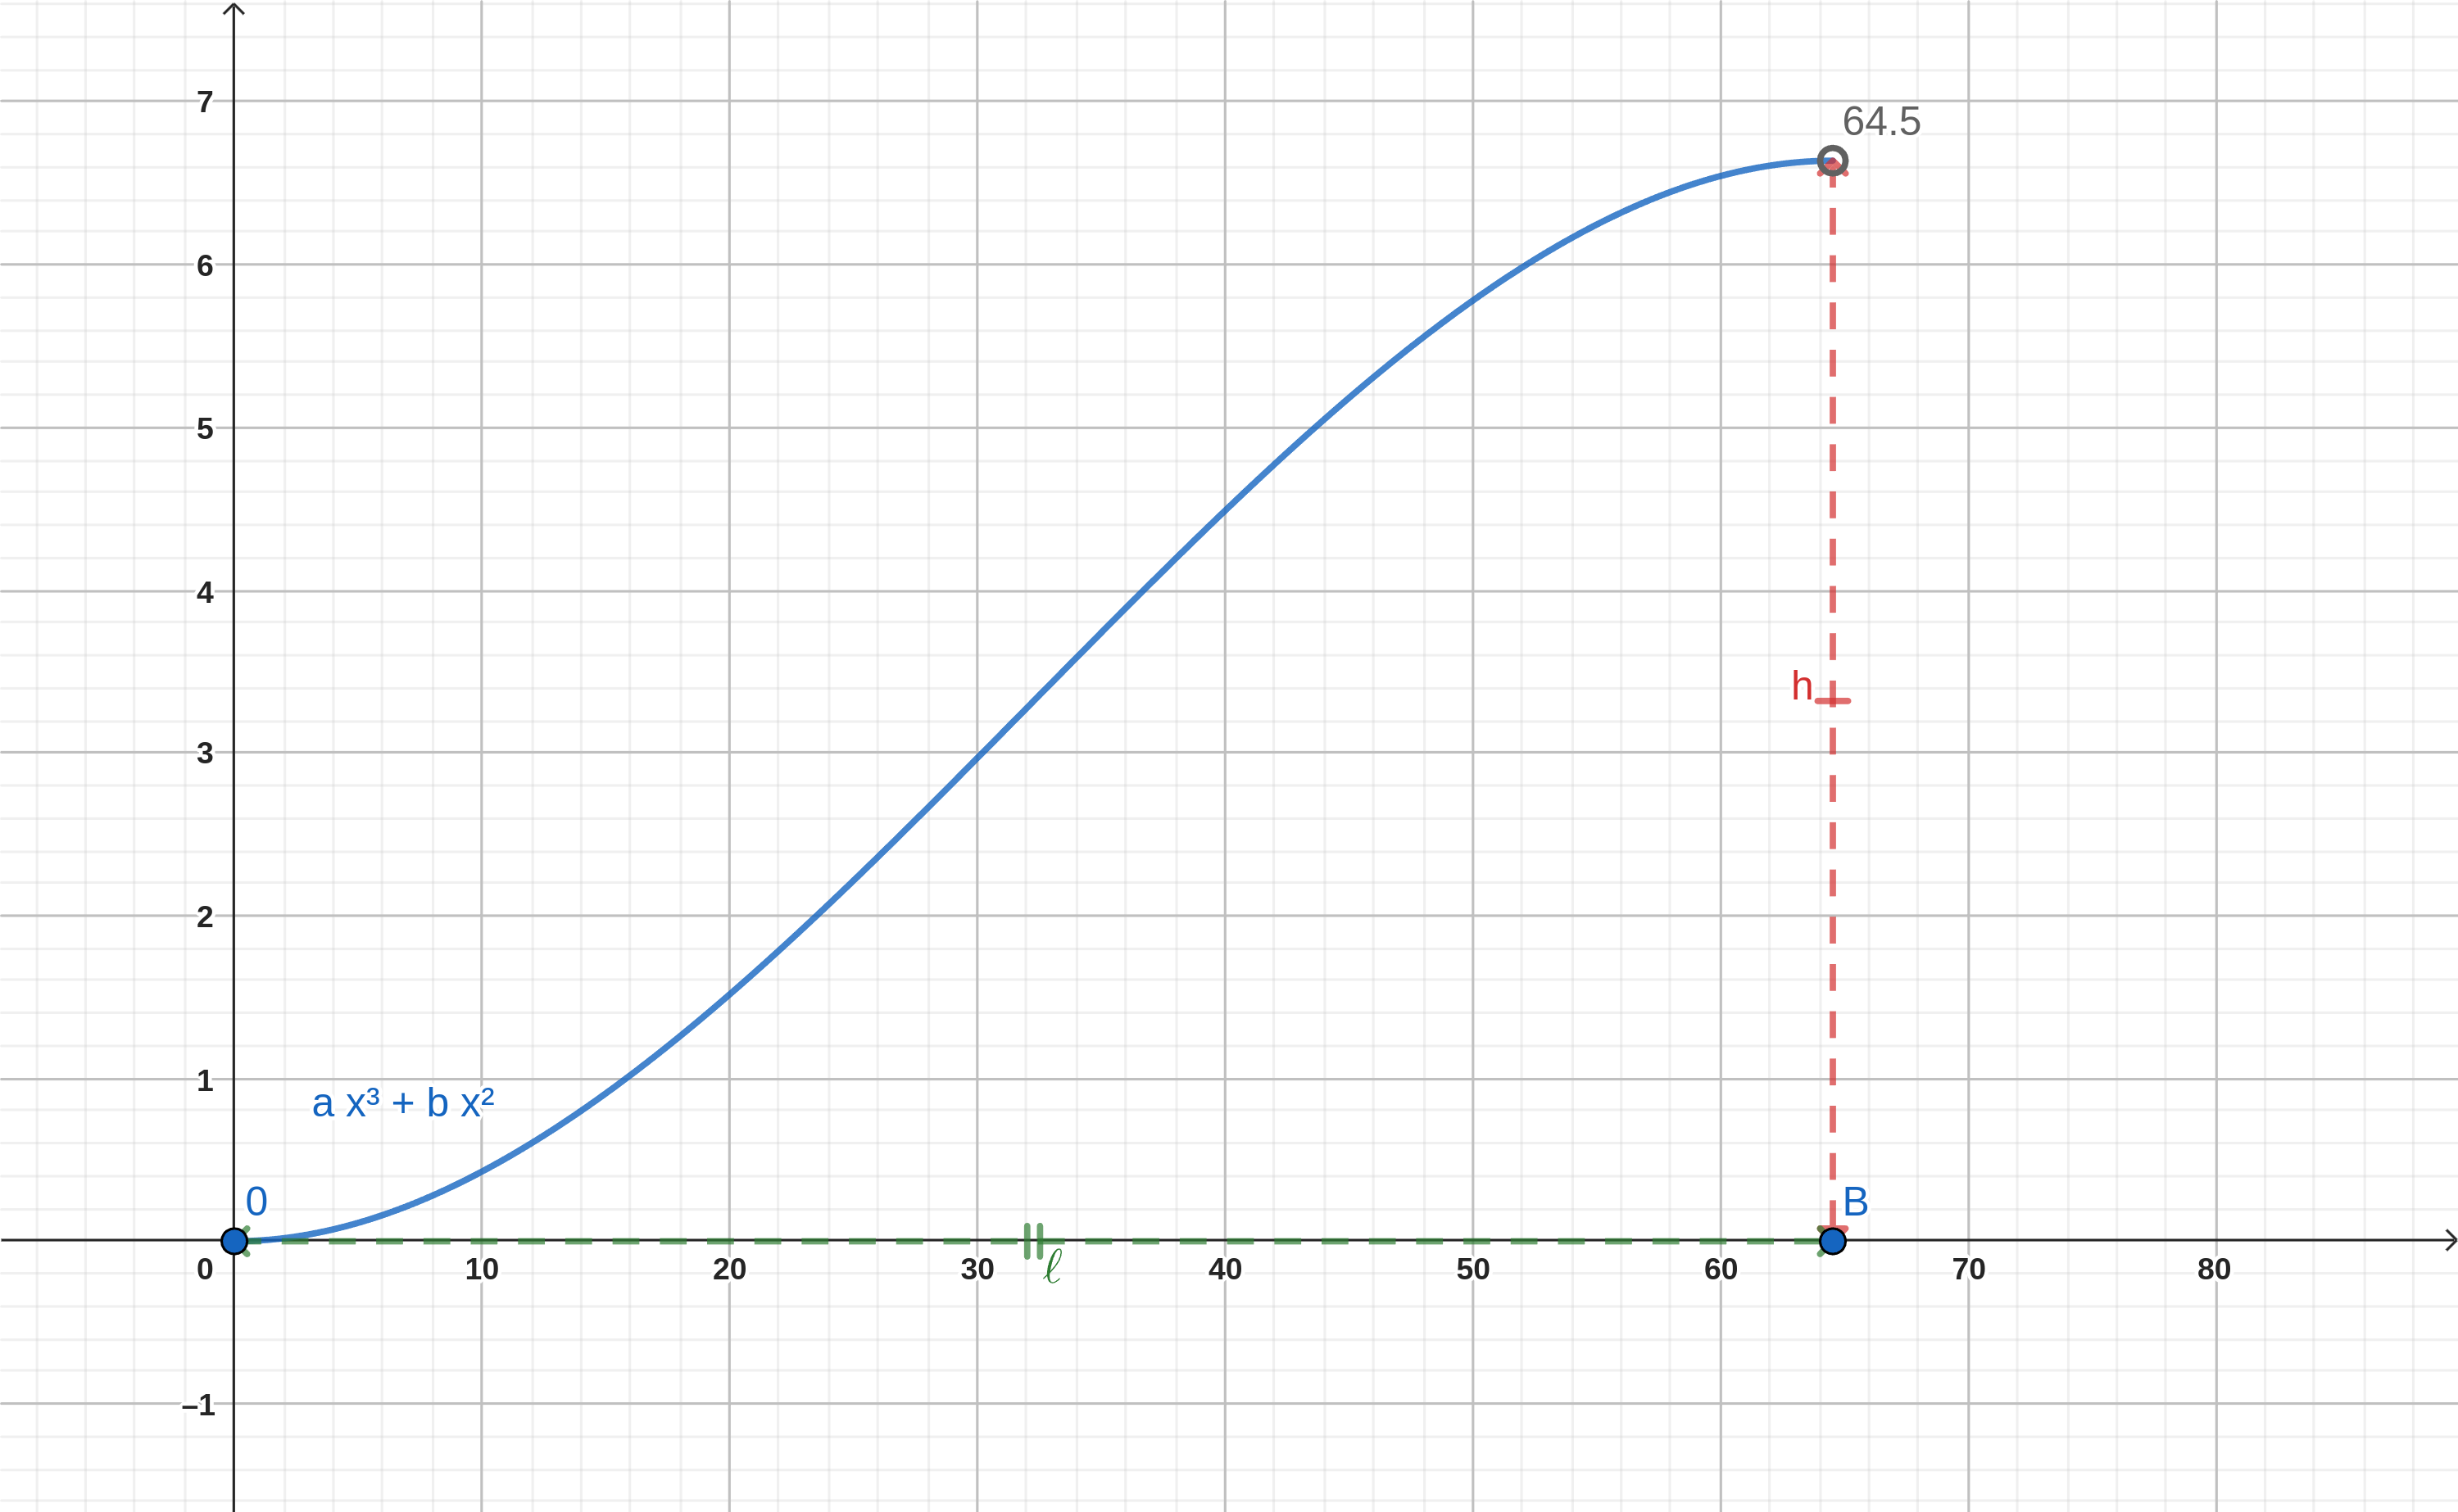
\includegraphics[height = 0.4\textheight]{recursos/geogebra-export-piloto.png}
\end{figure}